%=================================================================
% Modèle de devoir - Version française
% Auteur : <Votre nom>
% Description : Modèle LaTeX pour soumissions de devoirs
%=================================================================

\documentclass[12.0 pt,a4paper]{article}

 
%---------------------------------------------------------------
% PACKAGES
%---------------------------------------------------------------
\usepackage[T1]{fontenc}              % Encodage correct
\usepackage[utf8]{inputenc}           % Support UTF-8
\usepackage[french]{babel}            % Langue française
\usepackage{geometry}                 % Marges
\geometry{margin=2.0cm}
\usepackage{ amssymb }
\usepackage{amsmath,amssymb,amsthm}   % Math
\usepackage{graphicx}                 % Images
\usepackage{array}                    % Tableaux avancés
\usepackage{tikz}                     % K-maps, circuits logiques
\usetikzlibrary{matrix, positioning, automata, positioning, arrows.meta}  % Bibliothèques TikZ nécessaires

\usepackage{caption}                  % Légendes personnalisées
\usepackage{multirow}                 % Cellules multi-lignes
\usepackage{xcolor}                   % Couleurs
\usepackage{fancyhdr}                 % En-têtes / pieds de page

\usepackage{pdfpages}

\usepackage{import}
\usepackage{hyperref}                 % Liens hypertextes
\usepackage{float}                    % Placement précis
\usepackage{datetime}                 % Formatage de dates
\usetikzlibrary{calc}
\usepackage{tabu}
\usetikzlibrary{shapes, arrows, positioning}
\usepackage{changepage} % allows local margin changes
\usepackage{subfigure}
\usepackage{listings}
%---------------------------------------------------------------
% INFORMATIONS DU COURS ET DU GROUPE
%---------------------------------------------------------------
\newcommand{\codeclasse}{ELE140}                     % Code du cours
\newcommand{\nomclasse}{Conception des systèmes numériques} % Nom du cours
\newcommand{\titredevoir}{Devoir 2} % Titre du devoir
\newcommand{\groupe}{01}
\newcommand{\enseignant}{François Blanchard}
\newcommand{\datedepot}{\today}
\newcommand{\Session}{A25}
\newcommand{\auteurs}{
	Ourania Voyatzis~(VOYO78260401)\\
	Jhermain Louis-Jean~(LOUJ67360401)}

%---------------------------------------------------------------
% MISE EN PAGE
%---------------------------------------------------------------
\pagestyle{fancy}
\fancyhead[L]{\codeclasse\groupe}
\fancyhead[C]{\titredevoir}
\fancyhead[R]{\thepage}
\fancyfoot{}

%---------------------------------------------------------------
% DÉBUT DU DOCUMENT
%---------------------------------------------------------------
\begin{document}
	\begin{titlepage}
		\vspace*{\fill} 
		\centering
		{ \textbf{\nomclasse\ (\codeclasse)}}\\[0.5em]
		{ \textbf{\titredevoir}}\\[0.5em]
		\textbf{Enseignant :} \enseignant \\[1em]
		\textbf{Groupe :} \groupe \\[0.5em]
		\textbf{Remis par :}\\[0.5em]
		\auteurs \\[1.0em]
		\textbf{Date :} \datedepot
		\vspace*{\fill}
	\end{titlepage}
	\section*{Q.1 a)}
\subsection*{Assignement des Bascules: "simplest"}
\begin{figure}[H]
\centering{\begin{tabular}{|c|c|}
	\hline
	INIT & 000 \\
	\hline
	X1 & 001 \\
	\hline
	X2 & 010 \\
	\hline
	X3 & 011 \\
	\hline
	X4 & 100 \\
	\hline
	OK & 101 \\
	\hline
\end{tabular}}
\end{figure}

\subsection*{Diagramme d'états}
\begin{figure}[H]
	\centering
	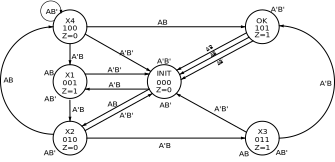
\includegraphics[width=0.7\linewidth]{BRUH}
\end{figure}
\subsection*{Table de transitions}
\begin{figure}[H]
	\centering{\begin{tabular}{|c|c|c|c|c|c|}
			\hline
			\rule[-1ex]{0pt}{2.5ex}  & \multicolumn{4}{c|}{AB} & Z \\
			\hline
			\rule[-1ex]{0pt}{2.5ex} Q2,Q1,Q0 & 00 & 01 & 11 & 10 &  \\
			\hline
			\rule[-1ex]{0pt}{2.5ex} 000 & 000 & 001 & 010 & 000 & 0 \\
			\hline
			\rule[-1ex]{0pt}{2.5ex} 001 & 000 & 010 & 001 & 001 & 1 \\
			\hline
			\rule[-1ex]{0pt}{2.5ex} 010 & 000 & 011 & 100 & 010 & 0 \\
			\hline
			\rule[-1ex]{0pt}{2.5ex} 011 & 000 & 101 & 011 & 011 & 1 \\
			\hline
			\rule[-1ex]{0pt}{2.5ex} 100 & 000 & 001 & 101 & 100 & 0 \\
			\hline
			\rule[-1ex]{0pt}{2.5ex} 101 & 101 & 000 & 000 & 000 & 1 \\
			\hline
			\rule[-1ex]{0pt}{2.5ex}  & \multicolumn{4}{c|}{Q2*Q1*Q0*} &  \\
			\hline
	\end{tabular}}
\end{figure}

\section*{Tables de Karnaugh des Bascules (Combinatoire)}

\begin{figure}[H]
	\centering
		\subsection*{Q2*} % use subsection* to avoid numbering
	\begin{tikzpicture}
	\matrix (m) [matrix of nodes,
	nodes={draw, minimum size=1.2cm, anchor=center},
	column sep=-\pgflinewidth, row sep=-\pgflinewidth] {
		0 & 0 & 0 & 0 & X & X & 1 & 0 \\
		0 & 0 & 1 & 0 & X & X & 0 & 0 \\
		0 & 0 & 0 & 1 & X & X & 0 & 1 \\
		0 & 0 & 0 & 0 & X & X & 0 & 1 \\
	};
	\footnotesize
	\node[above=4pt of m-1-1] {$\overline{Q_2}\overline{Q_1}\overline{Q_0}$};
	\node[above=4pt of m-1-2] {$\overline{Q_2}\overline{Q_1}Q_0$};
	\node[above=4pt of m-1-3] {$\overline{Q_2}Q_1Q_0$};
	\node[above=4pt of m-1-4] {$\overline{Q_2}Q_1\overline{Q_0}$};
	\node[above=4pt of m-1-5] {$Q_2Q_1\overline{Q_0}$};
	\node[above=4pt of m-1-6] {$Q_2Q_1Q_0$};
	\node[above=4pt of m-1-7] {$Q_2\overline{Q_1}Q_0$};
	\node[above=4pt of m-1-8] {$Q_2\overline{Q_1}Q_0$};
	
	\node[left=4pt of m-1-1, rotate=90, anchor=south] {$\overline{A}\overline{B}$};
	\node[left=4pt of m-2-1, rotate=90, anchor=south] {$\overline{A}B$};
	\node[left=4pt of m-3-1, rotate=90, anchor=south] {$AB$};
	\node[left=4pt of m-4-1, rotate=90, anchor=south] {$A\overline{B}$};
\end{tikzpicture}
\caption*{$Q2^*(A, B, Q2, Q1, Q0) = A'B'Q2Q0 + A'BQ1Q0 + AQ2Q0' + ABQ1Q0'$}


		\subsection*{Q1*}
	\begin{tikzpicture}
	\matrix (m) [matrix of nodes,
	nodes={draw, minimum size=1.2cm, anchor=center},
	column sep=-\pgflinewidth, row sep=-\pgflinewidth] {
		0 & 0 & 0 & 0 & X & X & 0 & 0 \\
		0 & 1 & 0 & 1 & X & X & 0 & 0 \\
		1 & 0 & 1 & 0 & X & X & 0 & 0 \\
		0 & 0 & 1 & 1 & X & X & 0 & 0 \\
	};
	\footnotesize
	\node[above=4pt of m-1-1] {$\overline{Q_2}\overline{Q_1}\overline{Q_0}$};
	\node[above=4pt of m-1-2] {$\overline{Q_2}\overline{Q_1}Q_0$};
	\node[above=4pt of m-1-3] {$\overline{Q_2}Q_1Q_0$};
	\node[above=4pt of m-1-4] {$\overline{Q_2}Q_1\overline{Q_0}$};
	\node[above=4pt of m-1-5] {$Q_2Q_1\overline{Q_0}$};
	\node[above=4pt of m-1-6] {$Q_2Q_1Q_0$};
	\node[above=4pt of m-1-7] {$Q_2\overline{Q_1}Q_0$};
	\node[above=4pt of m-1-8] {$Q_2\overline{Q_1}Q_0$};
	
	\node[left=4pt of m-1-1, rotate=90, anchor=south] {$\overline{A}\overline{B}$};
	\node[left=4pt of m-2-1, rotate=90, anchor=south] {$\overline{A}B$};
	\node[left=4pt of m-3-1, rotate=90, anchor=south] {$AB$};
	\node[left=4pt of m-4-1, rotate=90, anchor=south] {$A\overline{B}$};
\end{tikzpicture}
\caption*{$Q1^*(A, B, Q2, Q1, Q0) = A'BQ2'Q1'Q0 + A'BQ1Q0' + AB'Q1 + ABQ2'Q1'Q0' + AQ1Q0$}
	\subsection*{Q0*}
	\begin{tikzpicture}
		\matrix (m) [matrix of nodes,
		nodes={draw, minimum size=1.2cm, anchor=center},
		column sep=-\pgflinewidth, row sep=-\pgflinewidth] {
			0 & 0 & 0 & 0 & X & X & 1 & 0 \\
			1 & 0 & 1 & 1 & X & X & 0 & 1 \\
			0 & 1 & 1 & 0 & X & X & 0 & 1 \\
			0 & 1 & 1 & 0 & X & X & 0 & 0 \\
		};
	\footnotesize
		\node[above=4pt of m-1-1] {$\overline{Q_2}\overline{Q_1}\overline{Q_0}$};
		\node[above=4pt of m-1-2] {$\overline{Q_2}\overline{Q_1}Q_0$};
		\node[above=4pt of m-1-3] {$\overline{Q_2}Q_1Q_0$};
		\node[above=4pt of m-1-4] {$\overline{Q_2}Q_1\overline{Q_0}$};
		\node[above=4pt of m-1-5] {$Q_2Q_1\overline{Q_0}$};
		\node[above=4pt of m-1-6] {$Q_2Q_1Q_0$};
		\node[above=4pt of m-1-7] {$Q_2\overline{Q_1}Q_0$};
		\node[above=4pt of m-1-8] {$Q_2\overline{Q_1}Q_0$};
		
		\node[left=4pt of m-1-1, rotate=90, anchor=south] {$\overline{A}\overline{B}$};
		\node[left=4pt of m-2-1, rotate=90, anchor=south] {$\overline{A}B$};
		\node[left=4pt of m-3-1, rotate=90, anchor=south] {$AB$};
		\node[left=4pt of m-4-1, rotate=90, anchor=south] {$A\overline{B}$};
	\end{tikzpicture}
	\caption*{$Q0^*(A, B, Q2, Q1, Q0) = A'B'Q2Q0 + A'BQ0' + AQ2'Q0 + BQ2Q0' + A'BQ1$}
\end{figure}
\section*{Q1 b)}
\subsection*{Table de transitions}
\begin{figure}[H]
	\centering{\begin{tabular}{|c|c|c|c|c|c|}
			\hline
			\rule[-1ex]{0pt}{2.5ex}  & \multicolumn{4}{c|}{AB} & Z \\
			\hline
			\rule[-1ex]{0pt}{2.5ex} Q2 Q1 Q0 & 00 & 01 & 11 & 10 &  \\
			\hline
			\rule[-1ex]{0pt}{2.5ex} 111 & 111 & 110 & 010 & 111 & 0 \\
			\hline
			\rule[-1ex]{0pt}{2.5ex} 011 & 111 & 010 & 011 & 011 & 1 \\
			\hline
			\rule[-1ex]{0pt}{2.5ex} 010 & 111 & 001 & 000 & 010 & 0 \\
			\hline
			\rule[-1ex]{0pt}{2.5ex} 001 & 111 & 100 & 001 & 001 & 1 \\
			\hline
			\rule[-1ex]{0pt}{2.5ex} 000 & 111 & 011 & 100 & 000 & 0 \\
			\hline
			\rule[-1ex]{0pt}{2.5ex} 100 & 100 & 111 & 111 & 111 & 1 \\
			\hline
			\rule[-1ex]{0pt}{2.5ex} 110 & 111 & 111 & 111 & 111 & 0 \\
			\hline
			\rule[-1ex]{0pt}{2.5ex} 101 & 111 & 111 & 111 & 111 & 0 \\
			\hline
			\rule[-1ex]{0pt}{2.5ex}  & \multicolumn{4}{c|}{Q2*Q1*Q0*} &  \\
			\hline
	\end{tabular}}
\end{figure}

\subsection*{Tables de Karnaugh des Bascules (Combinatoire) b)}
\paragraph*{}
Dans les états indéfinis (001,101), nous revenons à l'état initial (tout à 1) afin de minimiser les risques.
\begin{figure}[H]
	\centering
	\subsection*{Q2*} % use subsection* to avoid numbering
	\begin{tikzpicture}
		\matrix (m) [matrix of nodes,
		nodes={draw, minimum size=1.2cm, anchor=center},
		column sep=-\pgflinewidth, row sep=-\pgflinewidth] {
			1 & 1 & 1 & 1 & 1 & 1 & 1 & 1 \\
			0 & 1 & 0 & 0 & 1 & 1 & 1 & 1 \\
			1 & 0 & 0 & 0 & 1 & 0 & 1 & 1 \\
			0 & 0 & 0 & 0 & 1 & 1 & 1 & 1 \\
		};
		\footnotesize
		\node[above=4pt of m-1-1] {$\overline{Q_2}\overline{Q_1}\overline{Q_0}$};
		\node[above=4pt of m-1-2] {$\overline{Q_2}\overline{Q_1}Q_0$};
		\node[above=4pt of m-1-3] {$\overline{Q_2}Q_1Q_0$};
		\node[above=4pt of m-1-4] {$\overline{Q_2}Q_1\overline{Q_0}$};
		\node[above=4pt of m-1-5] {$Q_2Q_1\overline{Q_0}$};
		\node[above=4pt of m-1-6] {$Q_2Q_1Q_0$};
		\node[above=4pt of m-1-7] {$Q_2\overline{Q_1}Q_0$};
		\node[above=4pt of m-1-8] {$Q_2\overline{Q_1}Q_0$};
		
		\node[left=4pt of m-1-1, rotate=90, anchor=south] {$\overline{A}\overline{B}$};
		\node[left=4pt of m-2-1, rotate=90, anchor=south] {$\overline{A}B$};
		\node[left=4pt of m-3-1, rotate=90, anchor=south] {$AB$};
		\node[left=4pt of m-4-1, rotate=90, anchor=south] {$A\overline{B}$};
	\end{tikzpicture}
	\caption*{$Q2^*(A, B, Q2, Q1, Q0) = A'B' + A'Q1'Q0 + A'Q2 + B'Q2 + ABQ1'Q0' + Q2Q1' + Q2Q0'$}
\end{figure}
	
	\begin{figure}[H]
		\centering
	\subsection*{Q1*}

	\begin{tikzpicture}
		\matrix (m) [matrix of nodes,
		nodes={draw, minimum size=1.2cm, anchor=center},
		column sep=-\pgflinewidth, row sep=-\pgflinewidth] {
			1 & 1 & 1 & 1 & 1 & 1 & 1 & 0 \\
			1 & 0 & 1 & 0 & 1 & 1 & 1 & 1 \\
			0 & 0 & 1 & 0 & 1 & 1 & 1 & 1 \\
			0 & 0 & 1 & 1 & 1 & 1 & 1 & 1 \\
		};
		\footnotesize
		\node[above=4pt of m-1-1] {$\overline{Q_2}\overline{Q_1}\overline{Q_0}$};
		\node[above=4pt of m-1-2] {$\overline{Q_2}\overline{Q_1}Q_0$};
		\node[above=4pt of m-1-3] {$\overline{Q_2}Q_1Q_0$};
		\node[above=4pt of m-1-4] {$\overline{Q_2}Q_1\overline{Q_0}$};
		\node[above=4pt of m-1-5] {$Q_2Q_1\overline{Q_0}$};
		\node[above=4pt of m-1-6] {$Q_2Q_1Q_0$};
		\node[above=4pt of m-1-7] {$Q_2\overline{Q_1}Q_0$};
		\node[above=4pt of m-1-8] {$Q_2\overline{Q_1}Q_0$};
		
		\node[left=4pt of m-1-1, rotate=90, anchor=south] {$\overline{A}\overline{B}$};
		\node[left=4pt of m-2-1, rotate=90, anchor=south] {$\overline{A}B$};
		\node[left=4pt of m-3-1, rotate=90, anchor=south] {$AB$};
		\node[left=4pt of m-4-1, rotate=90, anchor=south] {$A\overline{B}$};
	\end{tikzpicture}
	\caption*{$Q1^*(A, B, Q2, Q1, Q0) = Q1Q0 + B'Q1 + AQ2 + A'Q2'Q1'Q0' + A'B'Q0 + BQ2$}
\end{figure}
		\begin{figure}[H]
		\centering
	\subsection*{Q0*}

	\begin{tikzpicture}
		\matrix (m) [matrix of nodes,
		nodes={draw, minimum size=1.2cm, anchor=center},
		column sep=-\pgflinewidth, row sep=-\pgflinewidth] {
			1 & 1 & 1 & 1 & 1 & 1 & 1 & 0 \\
			1 & 0 & 0 & 1 & 1 & 0 & 1 & 1 \\
			0 & 1 & 1 & 0 & 1 & 0 & 1 & 1 \\
			0 & 1 & 1 & 0 & 1 & 1 & 1 & 1 \\
		};
		\footnotesize
		\node[above=4pt of m-1-1] {$\overline{Q_2}\overline{Q_1}\overline{Q_0}$};
		\node[above=4pt of m-1-2] {$\overline{Q_2}\overline{Q_1}Q_0$};
		\node[above=4pt of m-1-3] {$\overline{Q_2}Q_1Q_0$};
		\node[above=4pt of m-1-4] {$\overline{Q_2}Q_1\overline{Q_0}$};
		\node[above=4pt of m-1-5] {$Q_2Q_1\overline{Q_0}$};
		\node[above=4pt of m-1-6] {$Q_2Q_1Q_0$};
		\node[above=4pt of m-1-7] {$Q_2\overline{Q_1}Q_0$};
		\node[above=4pt of m-1-8] {$Q_2\overline{Q_1}Q_0$};
		
		\node[left=4pt of m-1-1, rotate=90, anchor=south] {$\overline{A}\overline{B}$};
		\node[left=4pt of m-2-1, rotate=90, anchor=south] {$\overline{A}B$};
		\node[left=4pt of m-3-1, rotate=90, anchor=south] {$AB$};
		\node[left=4pt of m-4-1, rotate=90, anchor=south] {$A\overline{B}$};
	\end{tikzpicture}
	\caption{$Q0^*(A, B, Q2, Q1, Q0) = AQ2'Q0 + A'B'Q2' + Q2Q1'Q0 + B'Q2Q1 + A'BQ0' + AQ2Q0'$}
\end{figure}
\section*{Q1 c)}
\paragraph*{}
Dans ce cas, le premier circuit A possède le moins de portes logiques.

\section*{Q.2 a)}	
\subsection*{Étape 1}
\paragraph*{}
J'ai décidé de renommer d'abord les variables pour rendre le code plus lisible.
		\begin{figure}[H]\footnotesize
\begin{lstlisting}[language=vhdl]
library ieee;
use ieee.std_logic_1164.all;
entity MEFDev2 is
port(
CLK, A, RESET, ENABLE : in std_logic;
Z : out std_logic);
end MEFDev2;
architecture MEFDev2_arch of MEFDev2 is
signal Q, QF: std_logic_vector(2 downto 0);
signal Q0, Q2, Q1 : std_logic;
begin
Q0 <= '1' when Q(2 downto 1) ="01" and A = '1' else
'1' when A ='0' and Q(2 downto 1) ="00" else
'1' when Q(2 downto 1) = "10" and A ='1' else
'1' when Q(2 downto 1) ="11" and A ='0' else
'0';
Z <= Q(1) and not(Q(2)) and Q(0);
process(CLK,RESET)
begin
if RESET = '1' then
tic <= "000";
elsif rising_edge (CLK) then
if ENABLE = '1' then
Q <= QF;
end if;
end if;
end process;
Q1 <= (not(A) and Q(0) and not(Q(2))) or (Q(1) 
and not(Q(0))) or (Q(2) and not(Q(0)) and A);
QF <= Q2 & Q1 & Q0;
Q2 <= '0' when Q ="110" and A ='1' else
'0' when Q(2 downto 1) = "00" and A = '0' else
'0' when Q(1 downto 0)="00" and A = '0' else
'0' when Q(2) = '0' and Q(0) = '1' else
'1';
end MEFDev2_arch;
\end{lstlisting}
\end{figure}

\clearpage

	\subsection*{Étape 2: Q2Q1Q0 et Z}
	\paragraph*{}
	À partir des équations ci-dessus, nous pouvons déduire les tableaux et équations suivants :\\
	
	
	\begin{figure}[H]
		\centering
	
		\begin{minipage}{0.45\textwidth}
			\centering
			\subsection*{} % use subsection* to avoid numbering
			\caption*{Q2* = Q2Q0 + Q2'Q0'A + Q1Q0'A' + Q1'Q0'A }
			\begin{tikzpicture}
				\matrix (m) [matrix of nodes,
				nodes={draw, minimum size=0.95cm, anchor=center},
				column sep=-\pgflinewidth, row sep=-\pgflinewidth] {
					0 & 1 & 0 & 0 \\
					1 & 1 & 0 & 0 \\
					1 & 0 & 1 & 1 \\
					0 & 1 & 1 & 1 \\
				};
				\node[above=4pt of m-1-1] {$\overline{Q_0}\overline{A}$};
				\node[above=4pt of m-1-2] {$\overline{Q_0}A$};
				\node[above=4pt of m-1-3] {$Q_0A$};
				\node[above=4pt of m-1-4] {$Q_0\overline{A}$};
				
				\node[left=4pt of m-1-1, rotate=90, anchor=south] {$\overline{Q_2}\overline{Q_1}$};
				\node[left=4pt of m-2-1, rotate=90, anchor=south] {$\overline{Q_2}Q_1$};
				\node[left=4pt of m-3-1, rotate=90, anchor=south] {$Q_2Q_1$};
				\node[left=4pt of m-4-1, rotate=90, anchor=south] {$Q_2\overline{Q_1}$};
			\end{tikzpicture}
			
		\end{minipage}
		\hfill\begin{minipage}{0.45\textwidth}
			\centering
			\subsection*{}
			\caption*{Q1* = Q2'Q0A' + Q1Q0' + Q2Q0'A }
			\begin{tikzpicture}
				\matrix (m) [matrix of nodes,
				nodes={draw, minimum size=0.95cm, anchor=center},
				column sep=-\pgflinewidth, row sep=-\pgflinewidth] {
					0 & 0 & 0 & 1 \\
					1 & 1 & 0 & 1 \\
					1 & 1 & 0 & 0 \\
					0 & 1 & 0 & 0 \\
				};
				\node[above=4pt of m-1-1] {$\overline{Q_0}\overline{A}$};
				\node[above=4pt of m-1-2] {$\overline{Q_0}A$};
				\node[above=4pt of m-1-3] {$Q_0A$};
				\node[above=4pt of m-1-4] {$Q_0\overline{A}$};
				
				\node[left=4pt of m-1-1, rotate=90, anchor=south] {$\overline{Q_2}\overline{Q_1}$};
				\node[left=4pt of m-2-1, rotate=90, anchor=south] {$\overline{Q_2}Q_1$};
				\node[left=4pt of m-3-1, rotate=90, anchor=south] {$Q_2Q_1$};
				\node[left=4pt of m-4-1, rotate=90, anchor=south] {$Q_2\overline{Q_1}$};
			\end{tikzpicture}
			
		\end{minipage}
		
	\end{figure}
	
	\subsection*{}
	\begin{figure}[H]
		\centering
		
		% ---------------- KMAP LEFT ----------------
		\begin{minipage}{0.45\textwidth}
			\centering
			\subsection*{} % use subsection* to avoid numbering
			\caption*{Q0* = Q2'Q1'A' + Q2'Q1A + Q2Q1A'}
			\begin{tikzpicture}
				\matrix (m) [matrix of nodes,
				nodes={draw, minimum size=0.95cm, anchor=center},
				column sep=-\pgflinewidth, row sep=-\pgflinewidth] {
					1 & 0 & 0 & 1 \\
					0 & 1 & 1 & 0 \\
					1 & 0 & 0 & 1 \\
					0 & 0 & 0 & 0 \\
				};
				\node[above=4pt of m-1-1] {$\overline{Q_0}\overline{A}$};
				\node[above=4pt of m-1-2] {$\overline{Q_0}A$};
				\node[above=4pt of m-1-3] {$Q_0A$};
				\node[above=4pt of m-1-4] {$Q_0\overline{A}$};
				
				\node[left=4pt of m-1-1, rotate=90, anchor=south] {$\overline{Q_2}\overline{Q_1}$};
				\node[left=4pt of m-2-1, rotate=90, anchor=south] {$\overline{Q_2}Q_1$};
				\node[left=4pt of m-3-1, rotate=90, anchor=south] {$Q_2Q_1$};
				\node[left=4pt of m-4-1, rotate=90, anchor=south] {$Q_2\overline{Q_1}$};
			\end{tikzpicture}
			
		\end{minipage}
\begin{minipage}{0.45\textwidth}
	\centering
	\subsection*{} % use subsection* to avoid numbering
	\caption*{Z = Q2'Q1Q0 }
	\begin{tikzpicture}
		\matrix (m) [matrix of nodes,
		nodes={draw, minimum size=0.95cm, anchor=center},
		column sep=-\pgflinewidth, row sep=-\pgflinewidth] {
			0 & 0 & 0 & 0 \\  % row for Q2=0
			0 & 0 & 1 & 0 \\  % row for Q2=1
		};
		% Column headers
		\node[above=4pt of m-1-1] {$\overline{Q_1}\overline{Q_0}$};
		\node[above=4pt of m-1-2] {$\overline{Q_1}Q_0$};
		\node[above=4pt of m-1-3] {$Q_1Q_0$};
		\node[above=4pt of m-1-4] {$Q_1\overline{Q_0}$};
		
		% Row labels
		\node[left=4pt of m-1-1, rotate=90, anchor=south] {$\overline{Q_2}$};
		\node[left=4pt of m-2-1, rotate=90, anchor=south] {$Q_2$};
	\end{tikzpicture}
\end{minipage}

		
	\end{figure}

\subsection*{Étape 3: Table de transition}
		\begin{figure}[H]
		\centering
	\begin{tabular}{|c|c|c| c|}
		\hline
		\rule[-1ex]{0pt}{2.5ex} {Q2*Q1*Q0*} & \multicolumn{2}{c|}{A} &  \\
		\hline
		\rule[-1ex]{0pt}{2.5ex} Q2Q1Q0 & 1 & 0 & Z\\
		\hline
		\rule[-1ex]{0pt}{2.5ex} 000 & 001 & 100 & 0 \\
		\hline
		\rule[-1ex]{0pt}{2.5ex} 001 & 011 & 000 & 0 \\
		\hline
		\rule[-1ex]{0pt}{2.5ex} 010 & 110 & 111 & 0 \\
		\hline
		\rule[-1ex]{0pt}{2.5ex} 011 & 010 & 001 & 1 \\
		\hline
		\rule[-1ex]{0pt}{2.5ex} 100 & 000 & 010 & 0 \\
		\hline
		\rule[-1ex]{0pt}{2.5ex} 101 & 100 & 100 & 0 \\
		\hline
		\rule[-1ex]{0pt}{2.5ex} 110 & 111 & 110 & 0 \\
		\hline
		\rule[-1ex]{0pt}{2.5ex} 111 & 101 & 100 & 0 \\
		\hline
	\end{tabular}
		\end{figure}

\subsection*{Étape 4: Diagramme d'état}
\begin{figure}[H]
	\centering
	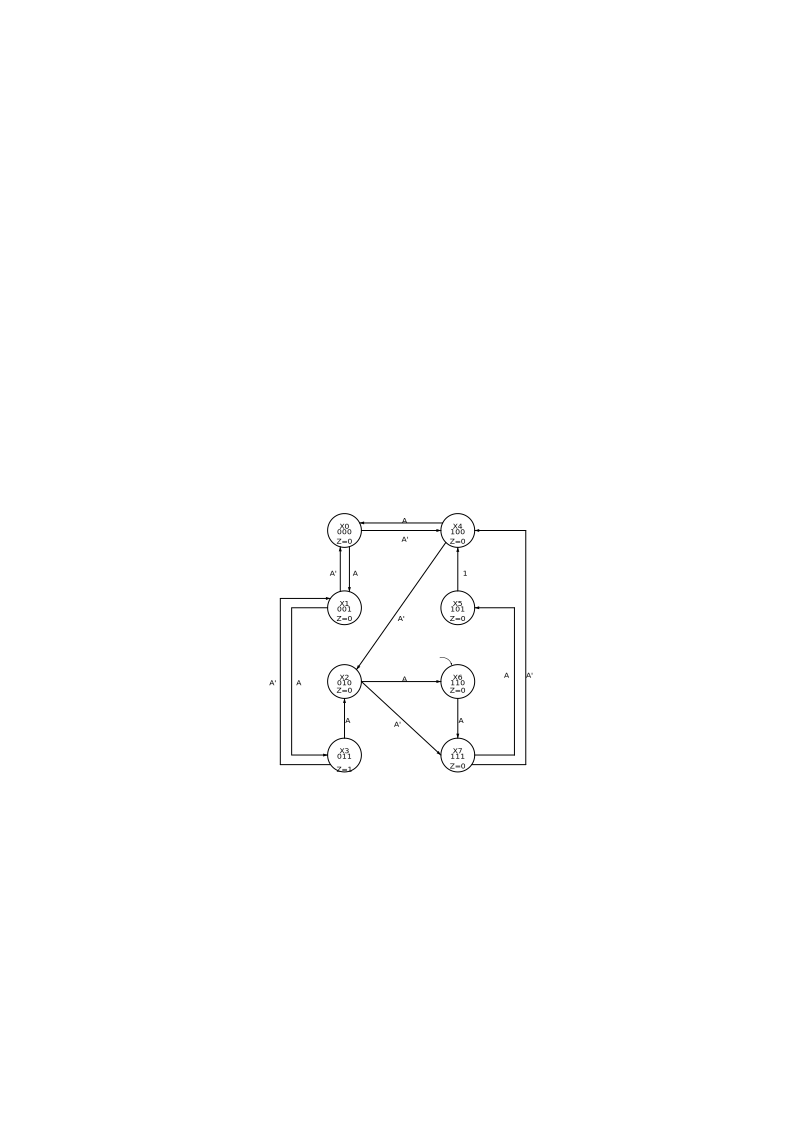
\includegraphics[width=0.5\linewidth]{Untitled}
	\caption{}

\end{figure}
\section*{Q2 b)}
\paragraph*{}
C'est un circuit de Moore car il n'a pas de signaux de rétroaction.
\section*{Q2 c)}
\paragraph*{}
Le code est très difficile à lire en raison des noms étranges ainsi que du fait que la logique combinatoire est divisée entre 2 blocs de code séparés, et ils ont utilisé inutilement des signaux binaires pour chaque bascule individuelle. Il y a peut-être encore plus de raisons pour lesquelles ce code ne suit pas les bonnes pratiques que j'ai peut-être manquées.
	
\end{document}